% !!!!!!!!!!!!!!!!!!   ВНИМАНИЕ !!!!!!!!!!!!!!!!!!!!!!!!!!!!!!!!!!!!!!!!!!!!!!!!!!!!!!!!!
% Заголовки разделов формируются при помощи команд \section{}, \subsection{}, \subsubsection{}
% Не используйте уровень вложенности заголовков больше трех!
% -----------------------------
% Для оформления теорем, лемм, следствий используйте окружения 
% Def     - Определение
% Teor    - Теорема
% Lem     - Лемма
% Predl   - Предложение
% Ass     - Утверждение
% Cor     - Следствие
% Example - Пример
% -----------------------------
% Доказательство теоремы начинается командой \proof и завершается командой \endproof
% -----------------------------
% Литература помещается в окружение biblio.

\documentclass[11pt, oneside, a4paper]{article}
%\usepackage[cp1251]{inputenc} % кодировка
\usepackage[utf8]{inputenc} % кодировка
\usepackage[english, russian]{babel} % Русские и английские переносы
\usepackage{graphicx}          % для включения графических изображений
\usepackage{cite}              % для корректного оформления литературы
\usepackage{enumitem}
\usepackage{amsmath,amsthm,amssymb}
\usepackage{mathtext}


%стилевой пакет
\usepackage{schoolseminar2022}


\begin{document}
% \udk     - универсальный десятичный классификатор
% \msc     -
% \title   - название статьи
% \authors - список авторов

\setcounter{page}{1}

\title{Разделение параметров в задачах глобальной оптимизации с помощью методов машинного обучения
\renewcommand{\thefootnote}{*}\footnote{Работа выполнена при поддержке Министерства науки и высшего образования РФ (проект \textnumero~0729-2020-0055) и научно-образовательного математического центра <<Математика технологий будущего>> (проект \textnumero~075-02-2021-1394).}}


\authors{К.А.~Баркалов, М.А.~Усова}
\organizations{Нижегородский государственный университет им. Н.И. Лобачевского \\ Нижний Новгород, Россия}



\abstractru{
В работе представлены результаты исследования подхода к решению задач глобальной оптимизации с разным характером зависимости от разных групп параметров.
Предложена схема выделения параметров задачи, которые оказывают локальное влияние на целевую функцию, что позволяет решать существенно многомерные задачи с использованием многошаговой схемы редукции размерности. При этом на разных уровнях рекурсии используются разные оптимизационные алгоритмы. Исследование работоспособности предложенного подхода проведено при решении тестовых и прикладных задач глобальной оптмизации.
}

\keywords{глобальная оптимизация, локальная оптимизация, редукция размерности, разделение параметров}


% \section{название} - заголовок раздела первого уровня
% \subsection{название} - заголовок раздела второго уровня
% \subsubsection{название} - заголовок раздела третьего уровня
% Не используйте уровень вложенности заголовков больше трех!
% Каждый абзац текста в статье начинается командой \par или пустой
% строкой.

\bigskip

\section{Постановка задачи}

В настоящее время методы глобальной оптимизации используются в различных областях науки и техники, например, для идентификации значений параметров математических моделей, при которых результаты моделирования наиболее близки к результатам, полученным экспериментально.
Число параметров, которые требуется определить подобным образом, например, для задач химической кинетики, может составлять десятки и сотни. В данном случае использование детерминированных методов глобальной оптимизации крайне ограничено в силу чрезвычайно больших вычислительных затрат на покрытие области поиска точками испытаний. Это остается справедливым даже в случае использования эффективных алгоритмов (например, \cite{Evtushenko2009,Paulavicius2016}), строящих существенно неравномерные покрытия. 
При этом частым явлением в подобных задачах является близкая к линейной зависимость по некоторой группе параметров, в то время как для остальных параметров наблюдается сложный многоэкстремальный характер. Заранее указать разделение на группы параметров с разным характером поведения целевой функции, как правило, не представляется возможным, т.к. целевая функция в обратных задачах задается как черный ящик. 

Задача многомерной многоэкстремальной оптимизации может быть определена как проблема поиска наименьшего значения действительной многоэкстремальной функции $\varphi(y)$
\begin{eqnarray}\label{main_problem}
& \varphi(y^\ast)=\min{\left\{\varphi(y): y\in D\right\}},  \\
& D=\left\{y\in R^N: a_i\leq y_i \leq b_i, 1\leq i \leq N\right\}, \nonumber
\end{eqnarray}
где $D$ есть область поиска, представляющая собой некоторый гиперпараллелепипед $N$-мерного евклидова пространства.
Будем предполагать, что функция $\varphi(y)$ задана в виде <<черного ящика>> и удовлетворяет условию Липшица
\[
\left|\varphi(y')-\varphi(y'')\right|\leq L\left\|y'-y''\right\|,\; y',y'' \in D,\; 0<L<\infty,
\]
с априори неизвестной константой $L$.
%Надо пояснить, что такое <<черный ящик>> - функция задается через алгоритм вычисления ее значений, аналитическая формула не известна. Алгоритм может быть сложным (решение СЛАУ или ОДУ), одно вычисление - трудоемкая операция.
%Пояснить смысл условия Липшица для прикладных задач - ограниченное изменение аргумента порождает ограниченное изменение значений функции.

Целевые функции большинства практических задач оптимизации обладают данным свойством.
Одновременно с этим будем предполагать, что зависимость целевой функции от $N_1$ параметров является многоэкстремальной, а от оставшихся $N_2 = N - N_1$ параметров зависимость является близкой к линейной или квадратичной. При этом разделение  параметров является неизвестным.

\section{Общее описание подхода к решению}

Решение поставленной задачи можно организовать с помощью \textit{многошаговой схемы редукции размерности} \cite{Grishagin2007}, согласно которой решение многомерной задачи оптимизации может быть получено посредством решения последовательности «вложенных» одномерных задач. Таким образом, решение исходной задачи (\ref{main_problem}) можно проводить следующим образом:
\begin{equation}\label{global_problem}
\varphi(y^*) = \min_{y\in D} \varphi (y) = \min_{y^1\in D_1} f(y^1), \; D_1=\left\{y\in R^{N_1}: 
a_i\leq y_i \leq b_i, \; 1\leq i \leq N_1\right\},
\end{equation}
где 
\begin{equation}\label{local_problem}
f(y^1) = \min_{ y^2 \in D_2} \varphi(y^1,y^2), \; D_2=\left\{y\in R^{N_2}: a_i\leq y_i \leq b_i, \; 
N_1+1\leq i \leq N\right\}. 
\end{equation}
Данный подход широко используется для снижения сложности алгоритмов глобальной оптимизации и позволяет формировать эффективные покрытия области поиска.
Решение  многоэкстремальной подзадачи (\ref{global_problem}), для которой требуется использовать сложные оптимизационные алгоритмы, будет проводиться на верхнем уровне рекурсии с помощью \textit{алгоритма глобального поиска} \cite{Strongin13}, принадлежащего классу характеристических алгоритмов, в сочетании со схемой редукции размерности на основе \textit{кривых Пеано} \cite{Sergeyev2013}. Этот алгоритм зарекомендовал себя как мощный инструмент для решения сложных многоэкстремальных задач.

Унимодальные подзадачи (\ref{local_problem}) на нижнем уровне могут быть решены с помощью методов прямого поиска, которые не предполагают гладкости функции.
При поиске минимума эти методы измеряют только значения функций, потому в отличие от методов типа BFGS, они не требуют вычисления градиента и хорошо работают в условиях наличия вычислительных ошибок в значениях функций, что является типичным при решении прикладных задач. Одним из наиболее популярных в практике методов этого класса является \textit{метод Хука-Дживса}, использующийся в нашем алгоритме. 

Описанный подход позволяет существенно снизить вычислительную сложность поиска оптимума. Однако его использование, вообще говоря, требует ручного распределения переменных по уровням, что, как уже отмечалось ранее, в практических задачах редко осуществимо. Потому возникла необходимость разработки схемы распределения параметров по уровням.

\section{Разделение параметров задачи}

Для разделения параметров задачи на локальные и глобальные предлагается следующая последовательность действий:

\textbf{Этап 1.} Зафиксировать опорную точку $\overline{y} = (\overline{y}_1, \overline{y}_2,...,\overline{y}_N)$ для целевой функции $\varphi(y)$ одним из следующих способов:
\begin{itemize}
\item точка фиксируется исходя из физического смысла решаемой прикладной задачи;
\item в качестве фиксированной точки используется решение, найденное локальным методом за $K$ итераций;
\item в качестве фиксированной точки используется решение, найденное глобальным методом за $K$ итераций.
\end{itemize}

\textbf{Этап 2.} Для всех компонент (переменных) $y_i, \; 1\leq i \leq N$ провести исследование на локальность:
\begin{enumerate}
\item вычислить $P+1$ значение целевой функции $\varphi(y)$ в точках $z_i^j = (\overline{y}_1,...,\overline{y}_{i-1},y_i^j,\overline{y}_{i+1},...,\overline{y}_N)$, где
$y_i^j =  a_i + jh, \; h=(b_i-a_i)/P, \; 0\leq j \leq P$;
\item сформировать множество $Q$, представляющее собой набор из $P+1$ пары вида $\left\{y_i^j, \varphi(z_i^j)\right\} $;
%Здесь вместо deg лучше бы использовать какое-то буквенное обозначение. Вроде бы, M у нас нигде здесь не задействовано. То есть, можно говорить о полиномем степени M
\item построить регрессионную модель заданной степени $deg$ на основе данных из $Q$;
\item вычислить оценку $R^2$ и провести классификацию i-й переменной:
\begin{itemize}
\item если $R^2$ больше заданного порога $T$, то добавить переменную к множеству локальных переменных,
\item иначе добавить переменную к множеству глобальных переменных.
\end{itemize}
\end{enumerate}

\begin{figure}[h!]
\centering 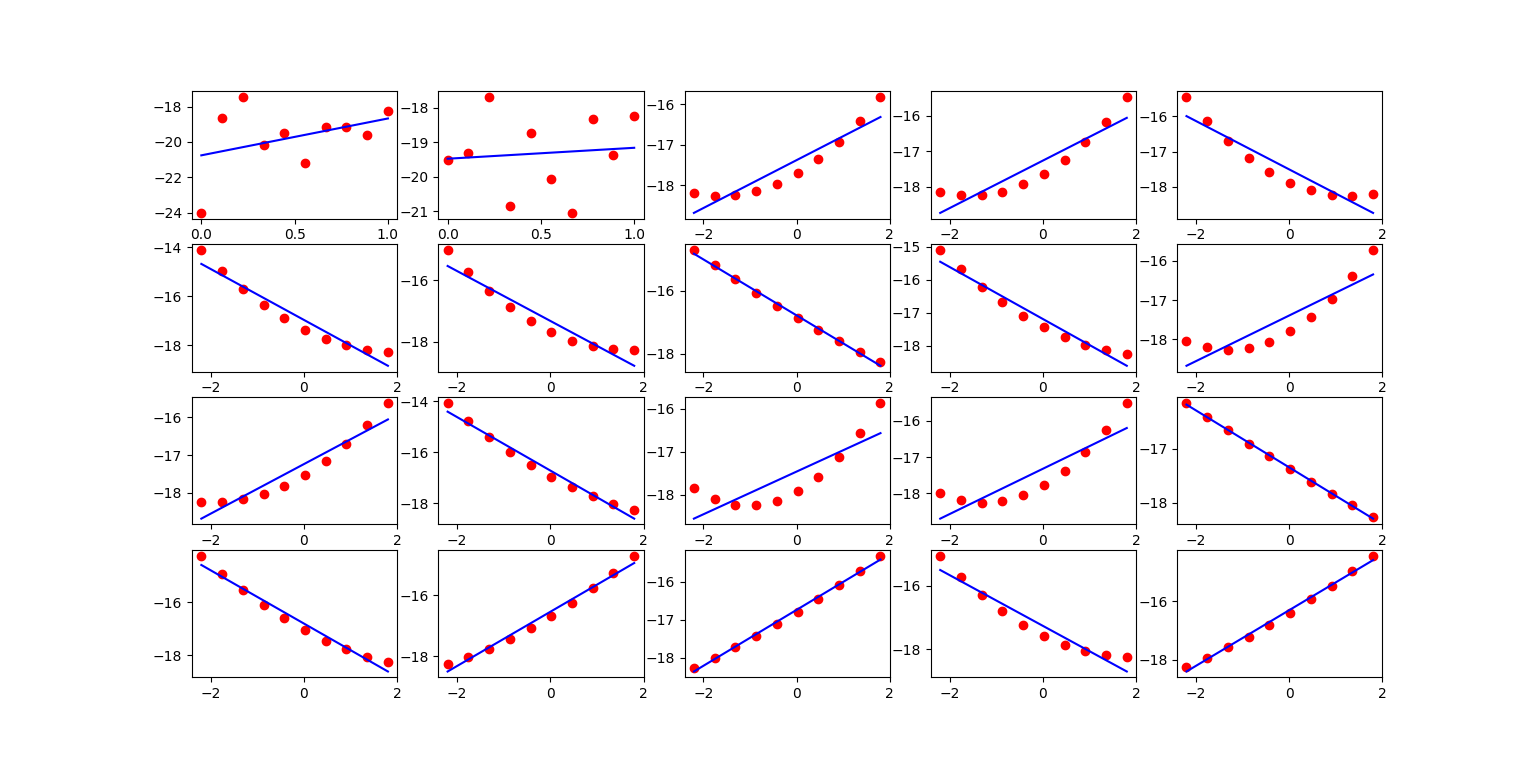
\includegraphics[width=1\linewidth]{regression_94}
\caption{Линейные регрессионные модели 20-мерной тестовой задачи  (2 глобальных параметра).}\label{regression_94_}
\end{figure}
\begin{figure}[h!]
\centering 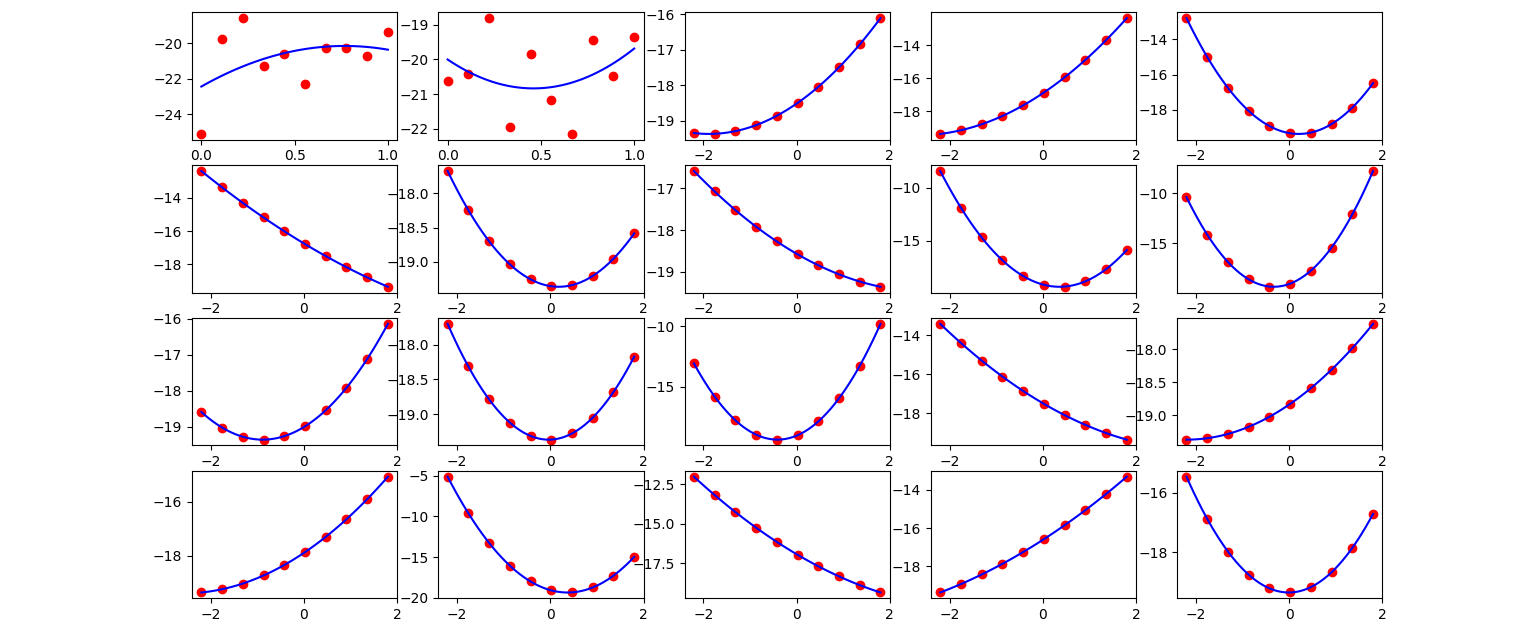
\includegraphics[width=1\linewidth]{regression_94_3}
\caption{Квадратичные регрессионные модели 20-мерной тестовой задачи (2 глобальных параметра).}\label{regression_94_3_}
\end{figure}

Значения  $K$, $deg$ и $T$ являются параметрами метода и устанавливаются исследователем в соответствии со свойствами решаемой задачей. В реализованном методе $deg = 1$ или $deg = 2$, что позволяет строить модель линейной или квадратичной регрессии соответственно.

В основе проводимой регрессии лежит \textit{метод наименьших квадратов} (МНК). Оценка качества построенной модели производится с помощью скорректированного коэффициента детерминации $R^2_a$, характеризующего схожесть построенной модели регрессии с целевой функцией в зафиксированном сечении. 

\textbf{Этап 3.} Если локальные переменные были обнаружены, то продолжить решение задачи с использованием описанной ранее многошаговой схемы. В противном случае запустить алгоритм глобального поиска, считая все переменные глобальными.

\section{Численные эксперименты}

Предложенный подход показал свою работоспособность при решении нескольких серий тестовых задач, представляющих собой линейные комбинации подзадач с глобальными параметрами и подзадач с локальными параметрами -- комбинации близких к линейным одномерных функций или функций с разным вкладом квадратичной составляющей.

\subsection{Описание серий задач}

В первом наборе тестовых задач (будем обозначать его GRIS-L) использовалось 20-мерные задачи комбинированного типа: локальная подзадача размерности 18, глобальная подзадача размерности 2. В качестве локальной составляющей использовались подзадачи, представляющие собой комбинацию близких к линейным одномерных функций:
\begin{equation}\label{X2_problem}
\varphi_j^{loc}(y) = \sum_{i=1}^{18} \left(M_{ij} y_i + L_{ij} y_i^2\right) ,
\end{equation}
где $-2.2 \leq y_i \leq 1.8$, а параметры $0.5 \leq |M_{ij}| \leq 1$ и $0.01 \leq L_{ij} \leq 0.3$  распределены случайно равномерно в соответствующих интервалах. В качестве глобальной составляющей задачи $\varphi_j^{glob}(y)$ использовались многоэкстремальные функции, предложенные Гришагиным \cite{Grishagin2001}.
\begin{figure}[h!]
\begin{minipage}{0.5\linewidth}
\center{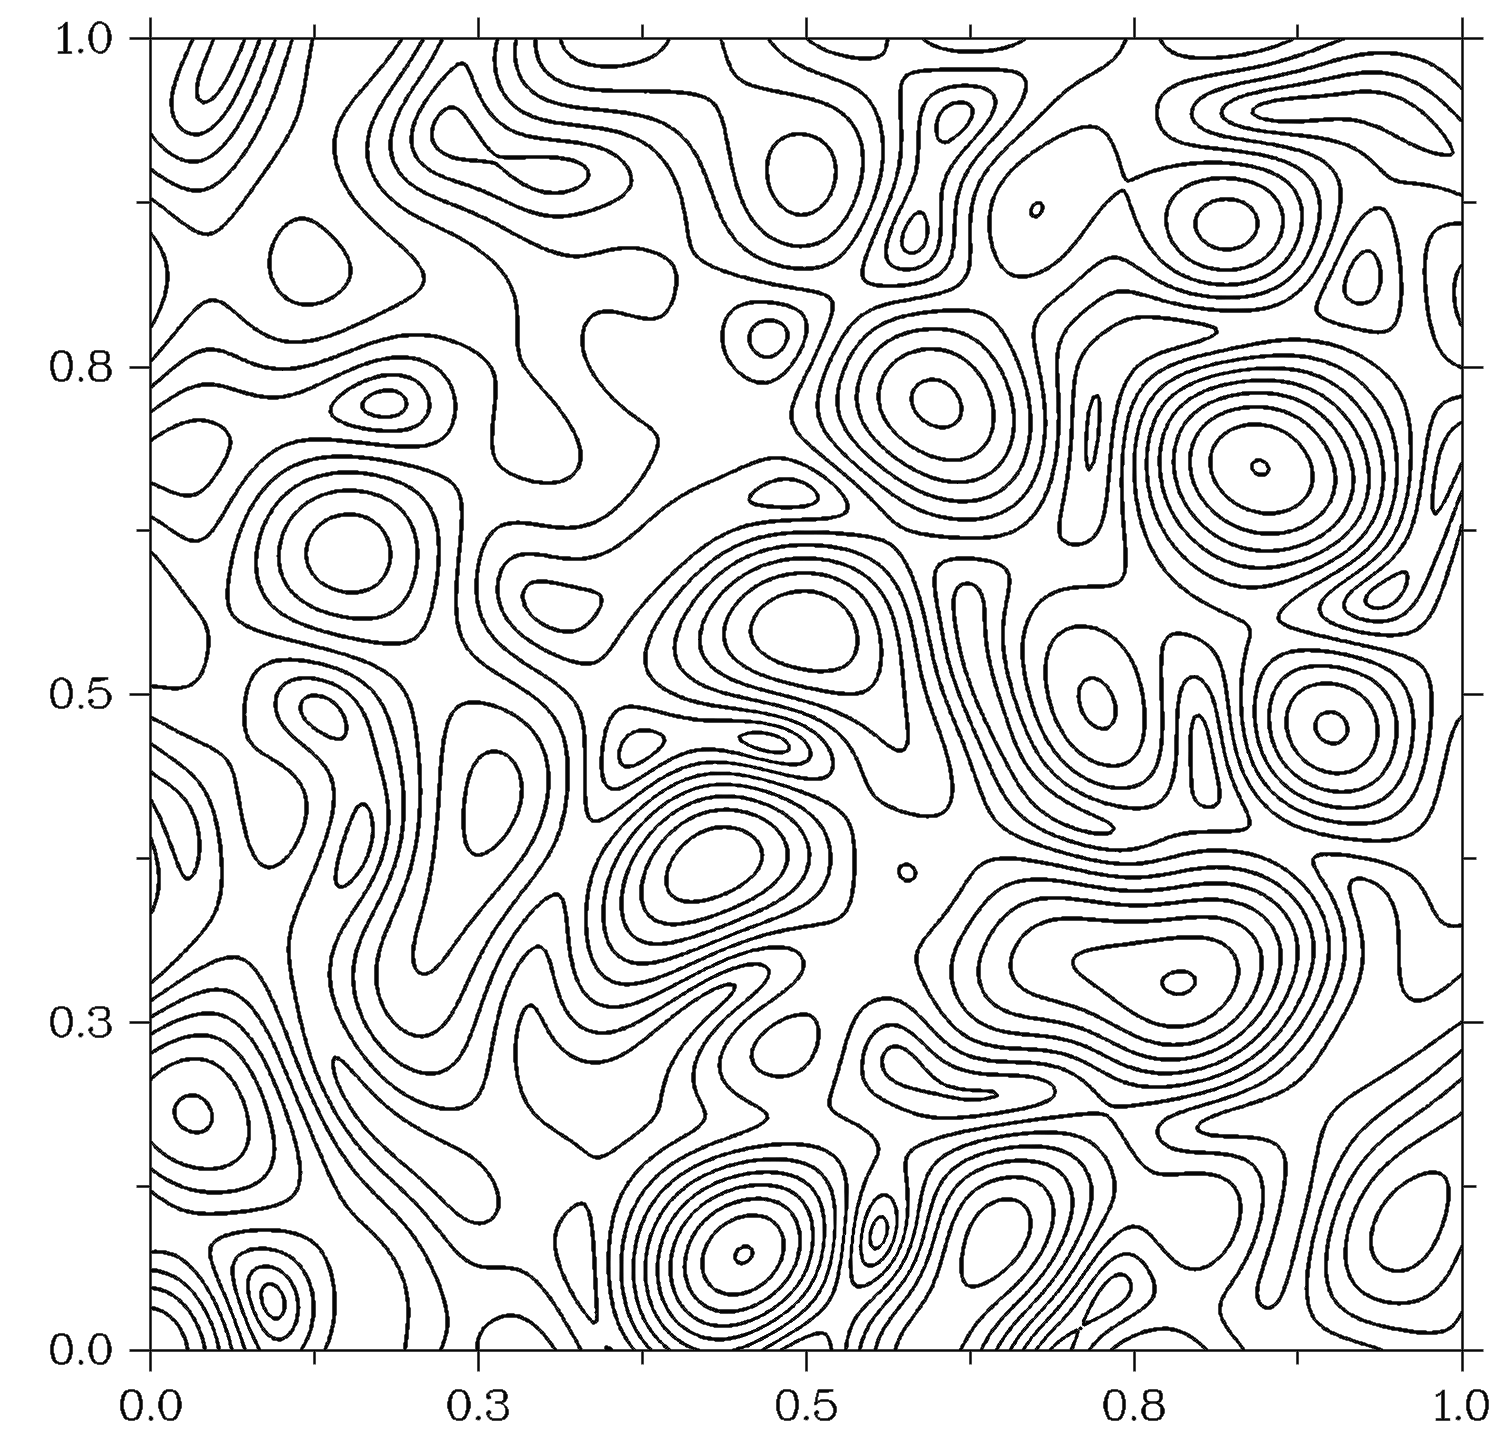
\includegraphics[width=1.0\linewidth]{fig1a.png}}
\end{minipage}
\begin{minipage}{0.5\linewidth}
\center{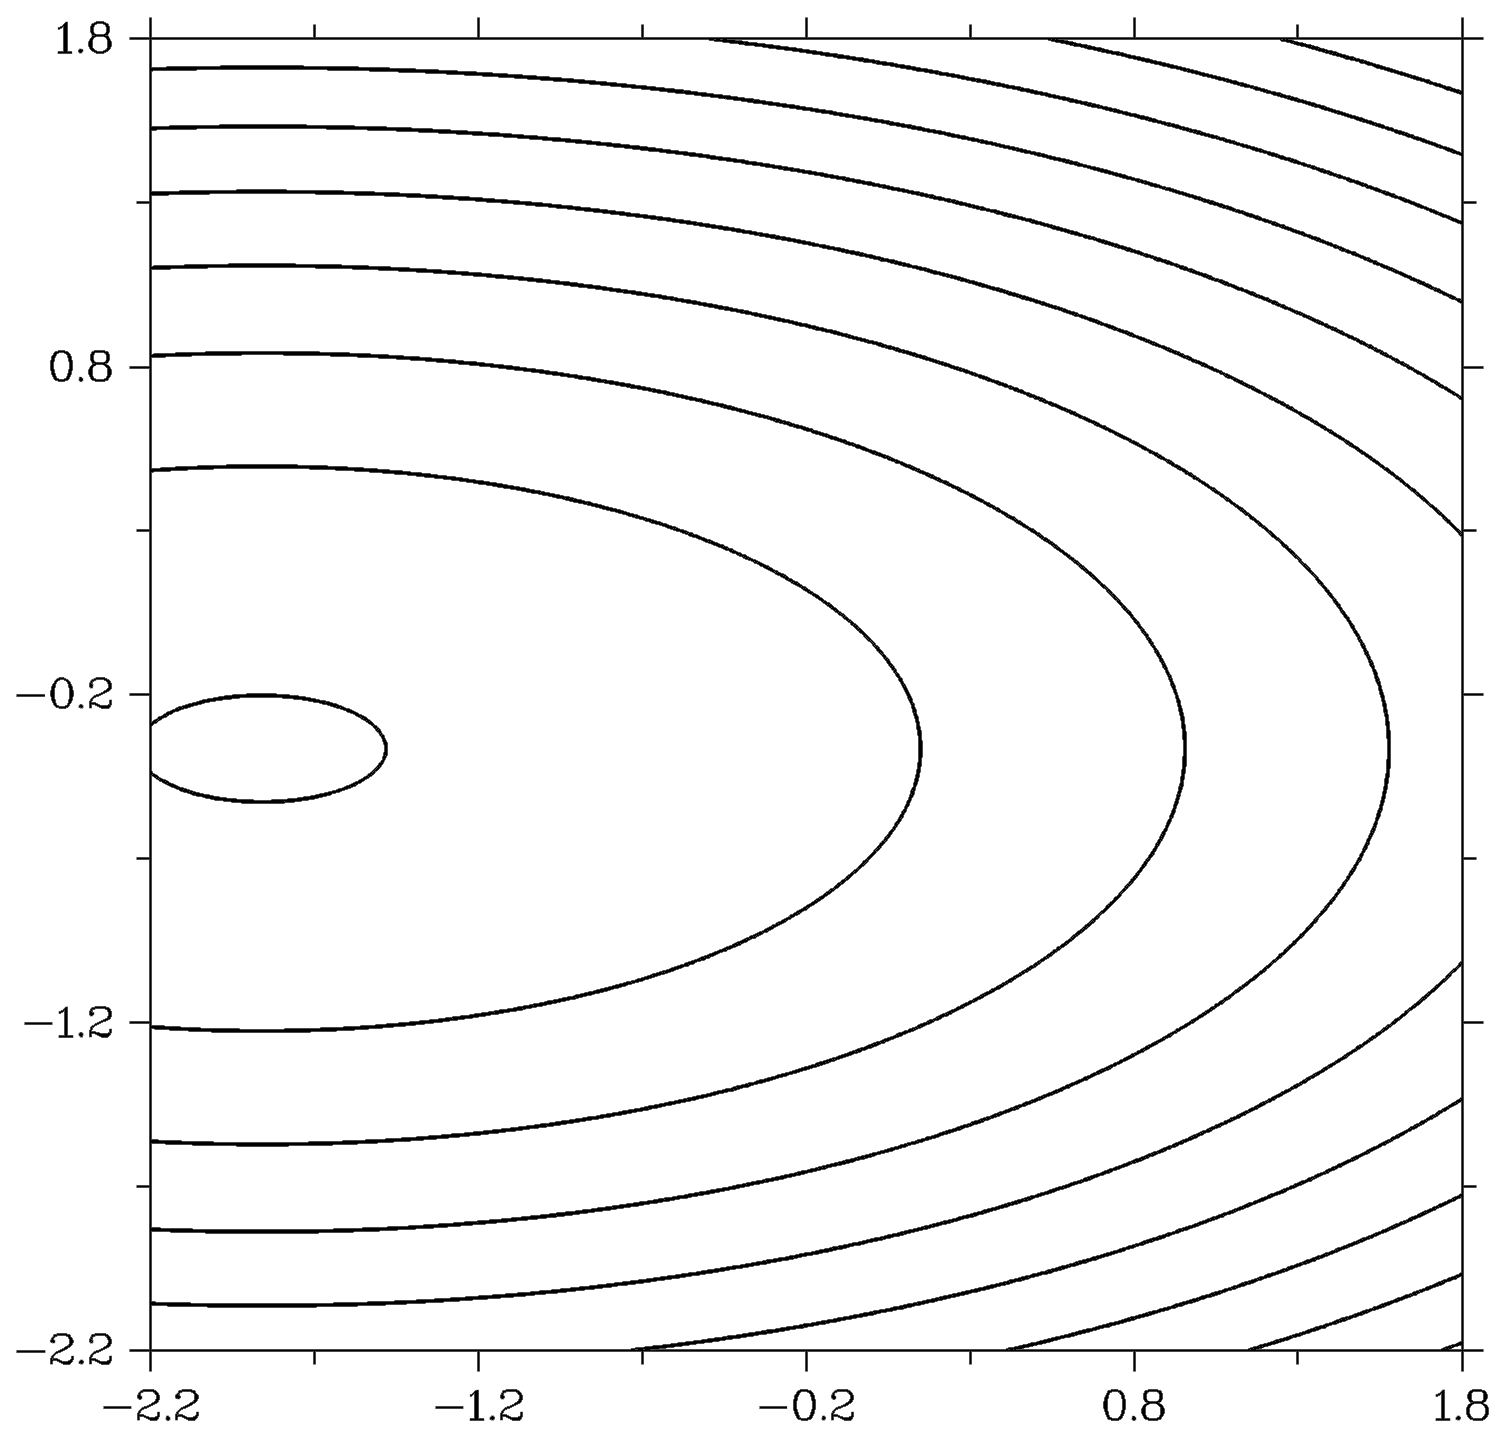
\includegraphics[width=1.0\linewidth]{fig1b.png}}
\end{minipage}
\caption{Линии уровня многоэкстремальной подзадачи и двумерное сечение локальной подзадачи.}
\label{fig}
\end{figure}
%\newpage
Целевая функция $\varphi(y)$ во всех наборах представляла собой линейную комбинацию подзадач, т.е. $\varphi_j(y) = \alpha \varphi_j^{glob}(y) + \beta \varphi_j^{loc}(y)$. Последовательность параметров в каждой задаче задавалась случайным образом. 

Во втором наборе задач (далее GRIS-LQ) параметры $M_{ij}$ и $L_{ij}$ локальной подзадачи (\ref{X2_problem}) были устроены таким образом, чтобы в 60\% случаев переменная имела несущественную квадратичную часть, в 30\% вклад квадратичной составляющей был существенным (как минимум, соизмеримым со вкладом линейной составляющей), а оставшиеся 10\% переменных были чисто линейными.

В третьей серии экспериментов (далее GKLS-L) в качестве многоэкстремальной части использовались 4-мерные функции из класса GKLS (функции Сергеева) \cite{Sergeyev2013} в качестве локальной составляющей использовалась локальные подзадачи серии GRIS-L.

\subsection{Результаты экспериментов на тестовых сериях}

По результатам экспериментов при решении серий задач с существенной многоэкстремальностью (GRIS-L и GRIS-LQ) было проведено корректное разделение на глобальные и локальные переменные, а затем задачи были успешно решены при помощи многошаговой схемы за приемлемое время и количество итераций.

Задачи с функциями GKLS для алгоритма являются более сложными, в силу схожести части параметров функций с параболоидами, поэтому решить все задачи серии за ограниченное количество итераций метода не удалось.

Вычисления проводились на компьютере с CPU Intel Core™ i7 10750H, 2.6 GHz. Исследуемый алгоритм был реализован на C++; вычисление значений целевой функции было реализовано в Python 3.9. Для построения и анализа регрессионной модели использовался пакет scikit-learn из Python.

Численные результаты серий экспериментов приведены в Таблице \ref{tab1}. В ней представлены данные о числе решенных задач $S$, среднем числе итераций глобального поиска на верхнем уровне рекурсии $G_{av}$, среднем числе испытаний на нижнем уровне $L_{av}$, среднем времени решения задачи $t_{av}$ (в секундах).

\begin{table}[ht]
	\caption{Результаты решения серий тестовых задач}
	\label{tab1}
	\begin{center}
		\begin{tabular}{ l c c c c c c } \hline
		 & $S$ &  $G_{av}$ &  $L_{av}$ & $t_{av}$ \\
    \hline
		GRIS-L & 20/20  & 705 &  378 545 & 1.3 \\
		GRIS-LQ & 20/20 & 705 &  420 397 & 1.4 \\
		GKLS-L & 18/20 & 9531 &  3 899 417 & 16.4 \\
		\hline
		\end{tabular}
	\end{center}
\end{table}

\subsection{Решение прикладной задачи}

В настоящее время наблюдается тенденция к улучшению экологических характеристик автомобильного топлива при сохранении высокого октанового числа. Алкилирование изобутана смешанными олефинами, катализируемое серной кислотой, позволяет получить высокооктановый компонент бензина с минимальным содержанием ароматических углеводородов. Для оптимизации описанного химического процесса в промышленности необходимо сначала разработать его модель, что в данном случае означает построение математической модели химического процесса, а затем его кинетической модели, т. е. численно рассчитать кинетические константы реакции.

Подробные описания моделей представлены в работе \cite{KinModel2022}. 

Аналитически узнать кинетические константы реакций, как правило, невозможно. В этом случае критерии качества найденного решения (целевая функция) не имеют явного аналитического описания, но допускают алгоритмическое представление и требуют значительных вычислительных ресурсов. Ранее использование параллельного асинхронного алгоритма, работающего на 8 узлах кластера, позволило значительно сократить время поиска оптимума. Для проведения указанного численного эксперимента использовался UNN supercomputer Lobachevsky (CentOS 7.2, SLURM, two CPU Intel Sandy Bridge E5-2660 2.2 GHz and 64 Gb RAM on the node). Найденные оптимальные параметры 15-мерной модели позволили адекватно смоделировать описанный процесс. При параметре метода  $r = 3$ было найдено лучшее значение целевой функции $0.519793$. Однако при использовании данного метода решения достигнуть заданной точности за обозримое время не представляется возможным (используется остановка по числу итераций или по ограничению времени решения).

С помощью исследуемого в данной работе метода за 15 часов было найдено улучшенное решение данной задачи -- $0.497063$. Размерность глобальной подзадачи -- $4$, число запусков глобального поиска -- $427$, число запусков локального метода -- $427 000$.

\begin{figure}[h!]
\begin{minipage}{0.5\linewidth}
\center{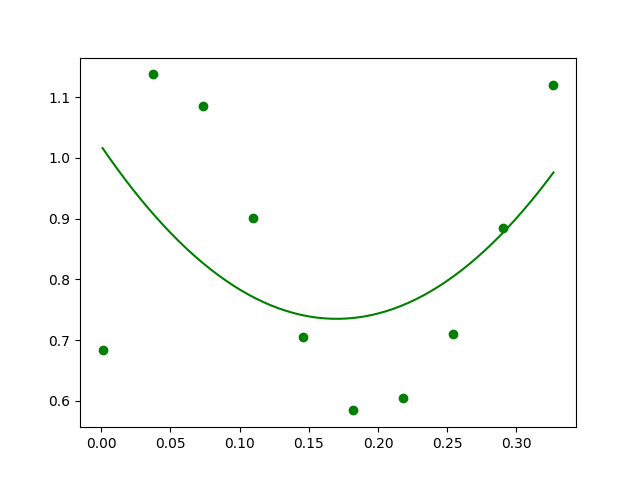
\includegraphics[width=1.0\linewidth]{saved_figure_2.png}}
\end{minipage}
\begin{minipage}{0.5\linewidth}
\center{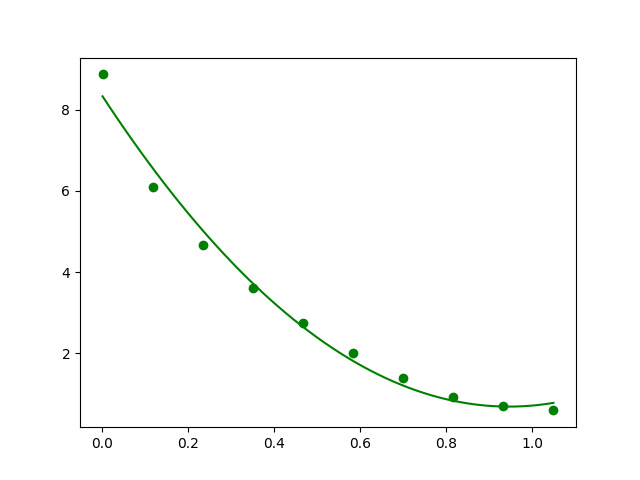
\includegraphics[width=1.0\linewidth]{saved_figure_8.png}}
\end{minipage}
\caption{Квадратичные регрессионные модели 15-мерной прикладной задачи глобального параметра (слева) и для локального параметра (справа).}
\label{fig}
\end{figure}

\section{Заключение}

В данной работе исследовался подход к разделению параметров по уровням для использования известной многоуровневой схемы редукции размерности в задачах глобальной оптимизации, комбинирующей использование кривых Пеано и многошаговую схему. Для решения редуцированных глобальных подзадач использовался алгоритм глобального поиска, для локальных подзадач был выбран метод Хука-Дживса. Предложена схема разделения параметров с использоваением построения регрессионной модели с помощью МНК. Проведены вычислительные эксперименты на серии тестовых задач большой размерности. Получено улучшенное решение прикладной задачи. Результаты экспериментов показывают, что предложенная схема позволяет корректно распределять параметры и эффективно находить оптимум задачи.

\begin{biblio}

\bibitem{Evtushenko2009} Евтушенко Ю. Г., Малкова В. У., Станевичюс А.-И. А. Параллельный поиск глобального экстремума функций многих переменных // {\it Журн. вычисл. матем. и матем. физ.} 2009. Т. 49. № 2. C. 255--269.

\bibitem{Paulavicius2016} Paulavi{\v c}ius R., {\v Z}ilinskas J. Advantages of Simplicial Partitioning for Lipschitz Optimization Problems with Linear Constraints // {\it Optim. Lett.} 2016. V. 10. No. 2. P. 237--246.

\bibitem{Grishagin2007} Городецкий С. Ю., Гришагин В. А. Нелинейное программирование и многоэкстремальная оптимизация. Н. Новгород: Изд-во ННГУ, 2007. 489 с.

\bibitem{Strongin13} Стронгин Р.Г., Гергель В.П., Гришагин В.А., Баркалов К.А. Параллельные вычисления в задачах глобальной оптимизации. М.: Изд-во МГУ, 2013. 280 с.

\bibitem{Sergeyev2013} Sergeyev, Y.~D. and Strongin, R.~G. and Lera, D. Introduction to global optimization exploiting space-filling curves // {\it Journal of Global Optimization}, Springer. 2013. V. 60, No. 3. P. 595--596.

\bibitem{Grishagin2001} Sergeyev Y., Grishagin V. Parallel Asynchronous Global Search and the Nested Optimization Scheme //  {\it J. Comput. Anal. Appl.} 2001. V. 3, No. 2. P. 123--145.

\bibitem{KinModel2022} Gubaydullin, I., Enikeeva, L., Barkalov, K., Lebedev, I., Silenko, D. Kinetic Modeling of Isobutane Alkylation with Mixed C4 Olefins and Sulfuric Acid as a Catalyst Using the Asynchronous Global Optimization Algorithm. // {\it Communications in Computer and Information Science}. 2022. V. 1618.  P. 293--306. 

%\bibitem{Sergeyev2008} Сергеев Я. Д., Квасов Д. Е. Диагональные методы глобальной оптимизации. М.: Физматлит, 2008. 352 с.


\end{biblio}

\newpage

\title{Separation of parameters using machine learning methods in global optimization problems}

\authors{K.A.~Barkalov,  M.A.~Usova}
\organizations{Lobachevsky State University of Nizhny Novgorod \\ Nizhny Novgorod, Russia}

% abstract is contained in the  abstract environment
\abstracten{
The paper presents the findings from research into an approach to solving global optimization problems with a different nature of dependence on diverse groups of parameters.
A scheme for choosing the problem parameters, which have a local effect on the objective function is proposed, which allows to solve essentially  multidimensional problems using the nested optimization scheme.
At the same time, different optimization algorithms are used at differing levels of recursion (nesting levels).
The proposed approach has demonstrated its efficiency in solving several series of test problems.
The effectiveness of the proposed approach was studied.}

\keywordsen{global optimization, local optimization, nested optimization scheme, high-dimensional problems, parameter separation}

\begin{biblioen}

\bibitem{Evtushenko2009} Evtushenko Yu. G., Malkova V. U., Stanevichyus A. A. Parallel global optimization of functions of several variables. // {\it USSR Computational Mathematics and Mathematical Physics} 2009. V. 49, No. 2. P. 255--269.

\bibitem{Paulavicius2016} Paulavi{\v c}ius R., {\v Z}ilinskas J. Advantages of Simplicial Partitioning for Lipschitz Optimization Problems with Linear Constraints // {\it Optim. Lett.} 2016. V. 10. No. 2. P. 237--246.

\bibitem{Grishagin2007} Gorodetskii S. Yu., Grishagin V. A. Nonlinear Programming and Optimization Multiextremal. Nizhny Novgorod, UNN Publ, 2007. 489 p.

\bibitem{Strongin13} Strongin, R.G., Gergel, V.P., Grishagin, V.A., Barkalov K.A. Parallel Computations in the Global Optimization Problems. Moscow, MSU Publ, 2012. 280 p.

\bibitem{Sergeyev2013} Sergeyev, Y.D. and Strongin, R.G. and Lera, D. Introduction to global optimization exploiting space-filling curves // {\it Journal of Global Optimization}, Springer. 2013. V. 60, No. 3. P. 595--596.

\bibitem{Grishagin2001} Sergeyev Y., Grishagin V. Parallel Asynchronous Global Search and the Nested Optimization Scheme // {\it J. Comput. Anal. Appl.} 2001. V. 3, No. 2. P. 123--145.

\bibitem{KinModel2022} Gubaydullin, I., Enikeeva, L., Barkalov, K., Lebedev, I., Silenko, D. Kinetic Modeling of Isobutane Alkylation with Mixed C4 Olefins and Sulfuric Acid as a Catalyst Using the Asynchronous Global Optimization Algorithm. // {\it Communications in Computer and Information Science}. 2022. V. 1618.  P. 293--306. 

\end{biblioen}

\end{document}
